\section{Memoria}

\subsection{Rol del Sistema Operativo}
El SO debe:
\begin{itemize}
    \item Llevar un registro de las partes de memoria que se estan utilizando y de aquellas que no.
    \item Asignar espacio en memoria principal a los procesos cuando estos la necesitan.
    \item Liberar espacio de memoria asignada a procesos que han terminado.
    \item Lograr que el programador se abstraiga de la alocacion de los programas.
    \item Brindar seguridad entre los procesos para que unos no accedan a secciones privadas de otros.
    \item Brindar la posibilidad de acceso compartido a determinadas secciones de la memoria.
    \item Garantizar la performance.
\end{itemize}

\subsection{Requisitos}
\begin{itemize}
    \item \textbf{Reubicacion}
    \begin{itemize}
        \item El programador no debe ocuparse de conocer donde sera colocado en la memoria RAM.
        \item Mientras un proceso se ejecuta, puede ser sacado y traido a la memoria (swap) y, posiblemente colocarse en diferentes direcciones.
        \item Las referencias a la memoria se deben "traducir" segun ubicacion actual del proceso.
    \end{itemize}
    \item \textbf{Proteccion}
    \begin{itemize}
        \item Los procesos NO deben referenciar/acceder a direcciones de memoria de otros procesos (salvo que tengan permiso).
        \item El chequeo se debe realizar durante la ejecucion.
    \end{itemize}
\item \textbf{Comparticion}
    \begin{itemize}
        \item Permitir que varios procesos accedan a la misma porcion de memoria.
        \item Permitir un mejor uso de la memoria principal, evitando copias innecesarias (repetidas) de instrucciones.
    \end{itemize}
\end{itemize}

\subsection{Direcciones}
\subsubsection{Espacio de direcciones}
\begin{itemize}
    \item Rango de direcciones (a memoria) posibles que un proceso puede utilizar para direccionar sus instrucciones y datos.
    \item Es independiente de la ubicacion "real" del proceso en la memoria RAM.
\end{itemize}

\subsection{Tipos de direcciones}
\begin{itemize}
    \item \textbf{Logicas/Virtuales}
    \begin{itemize}
        \item Referencia a una localidad de memoria.
        \item Representa una direccion en el "Espacio de Direcciones del Proceso".
    \end{itemize}
    \textbf{Fisicas}
    \begin{itemize}
        \item Referencia una localidad en la memoria principal.
    \end{itemize}
\end{itemize}
Es necesario algun tipo de conversion a de direcciones logicas a fisicas y viceversa.
\subsubsection{Conversion de Direcciones}
Una forma simple de realizar la conversion es utilizando registros auxiliares.
\begin{itemize}
    \item \textbf{Registro Base:} direccion de comienzo del Espacio de Direcciones del proceso en la memoria principal.
    \item \textbf{Registro Limite} direccion final del proceso o medida del proceso.
    \item Ambos valores se fijan cuando el espacio de direcciones del proceso es cargado a memoria.
    \item Varian entre procesos.
\end{itemize}
    Si la conversion se realiza en tiempo de ejecicion, las direcciones logicas se denominan \textbf{direcciones virtuales}, y son diferentes a las fisicas.
En este caso, el mapeo entre ambos tipos de direcciones se realiza por hardware, mediante la \textbf{Memory Management Unit (MMU)}.
\begin{figure}
    \begin{center}
        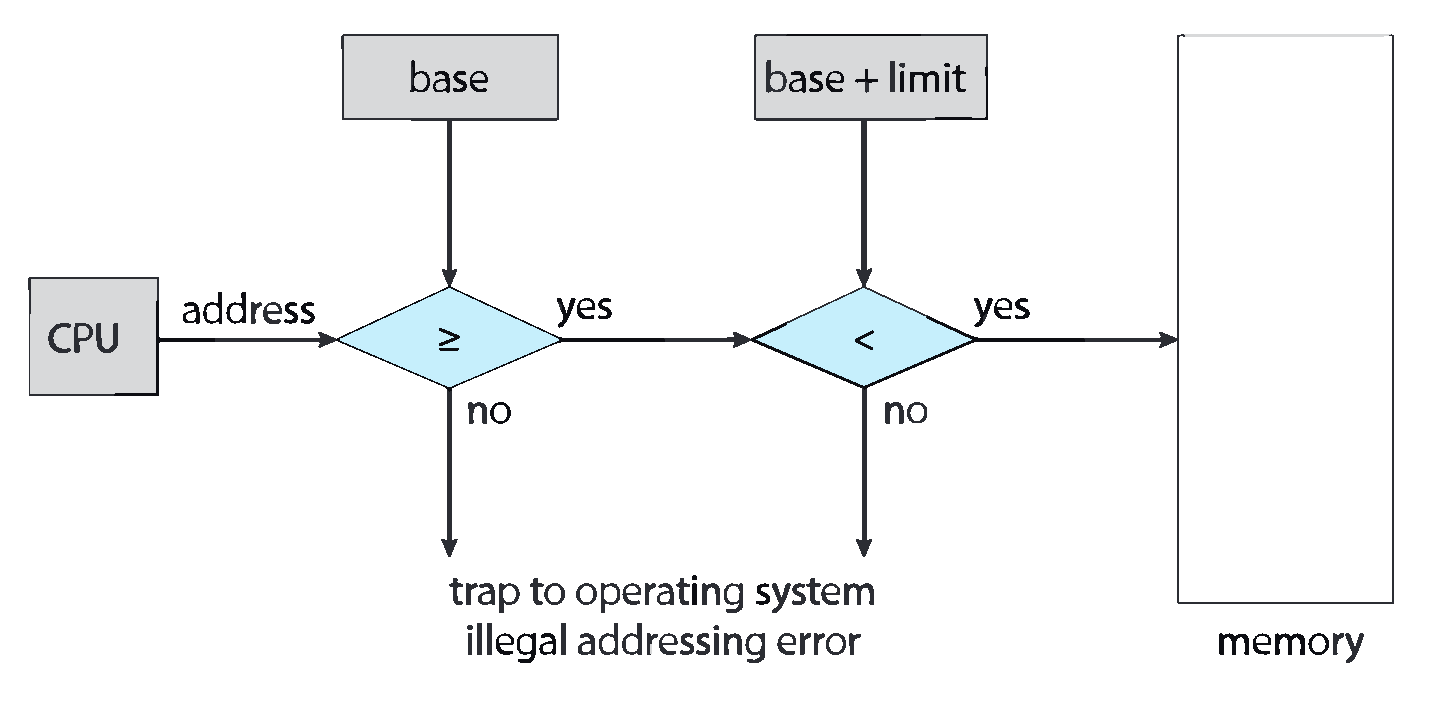
\includegraphics[width=0.75\textwidth]{assets/ConversionDirecciones.pdf}
    \end{center}
    \caption{Proteccion de direcciones mediante registros base y limite.}\label{fig:69}
\end{figure}

\subsection{Memory Management Unit (MMU)}
\begin{itemize}
    \item Es un dispositivo de hardware que mapea direcciones virtuales a fisicas.
    \item Es parte de la CPU.
    \item Reprogramarla es una operacion privilegiada.
    \item El valor en el "registro de realocacion" es sumado a cada direccion generada por el proceso de usuario al momento de aceder a la memoria.
    \item Los procesos solo utilizan direcciones virtuales.
\end{itemize}
\begin{figure}[h]
    \begin{center}
        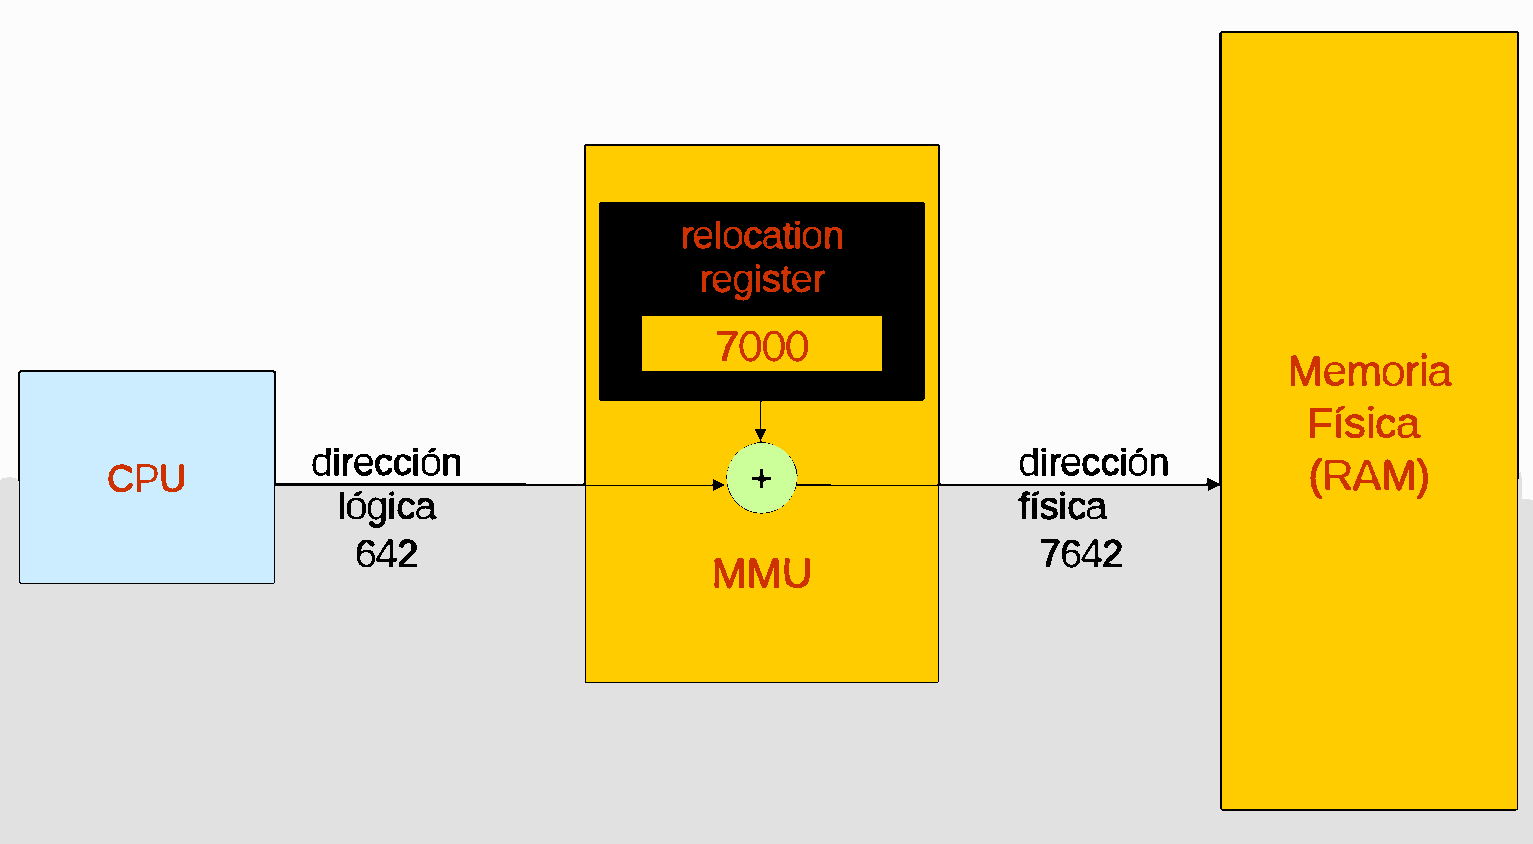
\includegraphics[width=0.70\textwidth]{assets/MMU.pdf}
    \end{center}
    \caption{Funcionamiento de la MMU}\label{fig:}
\end{figure}

\subsection{Mecanismos de asignacion de memoria}
\begin{itemize}
    \item \textbf{Parcitiones Fijas}
    \begin{itemize}
        \item La memoria se divide en particiones o regiones de tamaño fijo (de mismo tamaño o no).
        \item Alojan un proceso cada una.
        \item Cada proceso se coloca de acuerdo a algun criterio (worst-fit, best-fit ,etc).
    \end{itemize}
    \item \textbf{Parciciones Dinamicas}
    \begin{itemize}
        \item Las parcitiones varian en tamaño y numero.
        \item Alojan un proceso cada una.
        \item Cada particion se genera en forma dinamica, del tamaño exacto que necesita el proceso.
    \end{itemize}
\end{itemize}

\subsection{Fragmentacion}
La \textbf{fragmentacion} se produce cuando un alocalidad de memoria no puede ser utilizada por no encontrarse en forma continua.
Existen dos tipos:
\begin{itemize}
    \item \textbf{Fragmentacion Interna}
    \begin{itemize}
        \item Se produce en el esquema de particiones fijas.
        \item Es la porcion de la particion que queda sin utilizar.
    \end{itemize}
    \item \textbf{Fragmentacion Externa}
    \begin{itemize}
        \item Se produce en el esquema de particiones dinamicas.
        \item Son huecos que van quedando en la memoria a medida que los procesos finalizan.
        \item Al no encontrarse en forma contigua, puede darse el caso de que tengamos memoria libre para alocar un proceso, pero que no la podamos utilizar.
        \item Puede soucionarse utilizando la \textbf{compactacion}
    \end{itemize}
\end{itemize}

\subsection{Paginacion}
\begin{itemize}
    \item La memoria fisica es dividida logicamente en pequeños trozos de igual tamaño llamados \textbf{Marcos}.
    \item La memoria logica (espacio de direcciones) es dividida en trozos de igual tamaño que los marcos, llamados \textbf{Paginas}.
    \item El SO debe mantener una tabla de paginas por cada proceso, donde cada entrada contiene (entre otras), el Marco en el que se coloca cada pagina.
    \item La direccion logica se interpreta como un numero de pagina y un desplazamiento dentro de la misma.
\end{itemize}
\begin{figure}[h]
    \begin{center}
        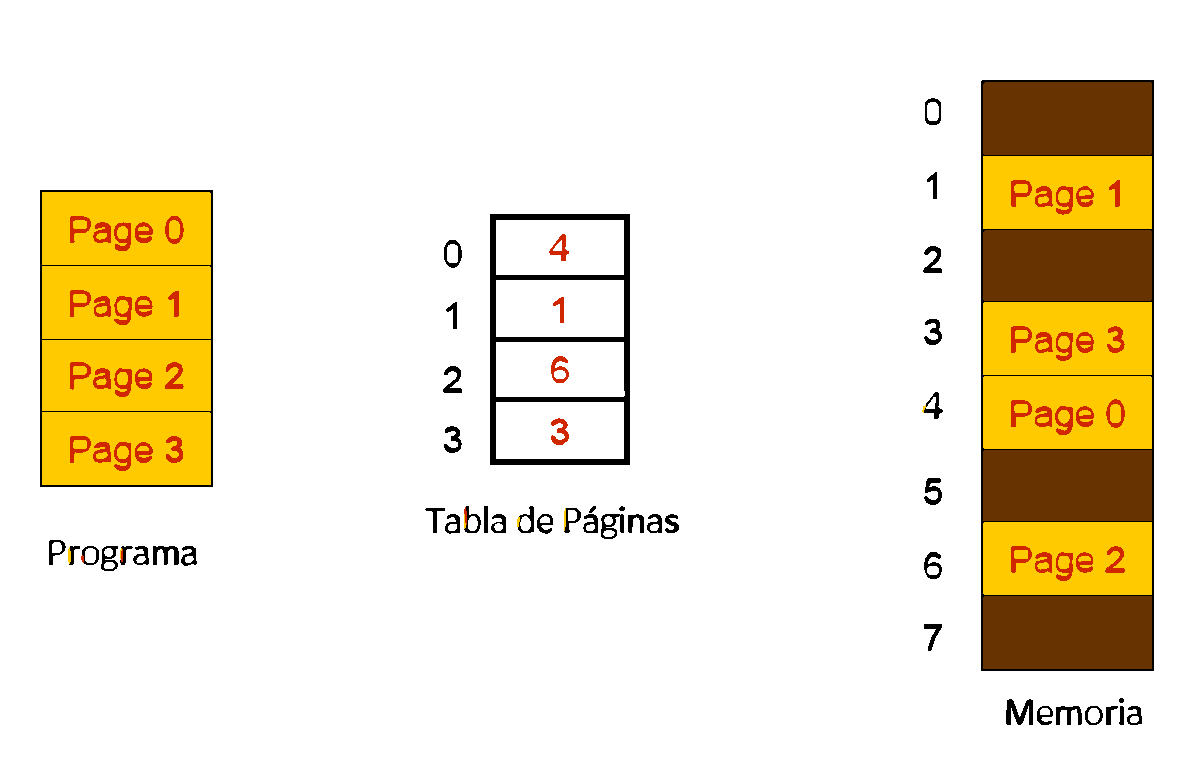
\includegraphics[width=0.70\textwidth]{assets/Paging.pdf}
        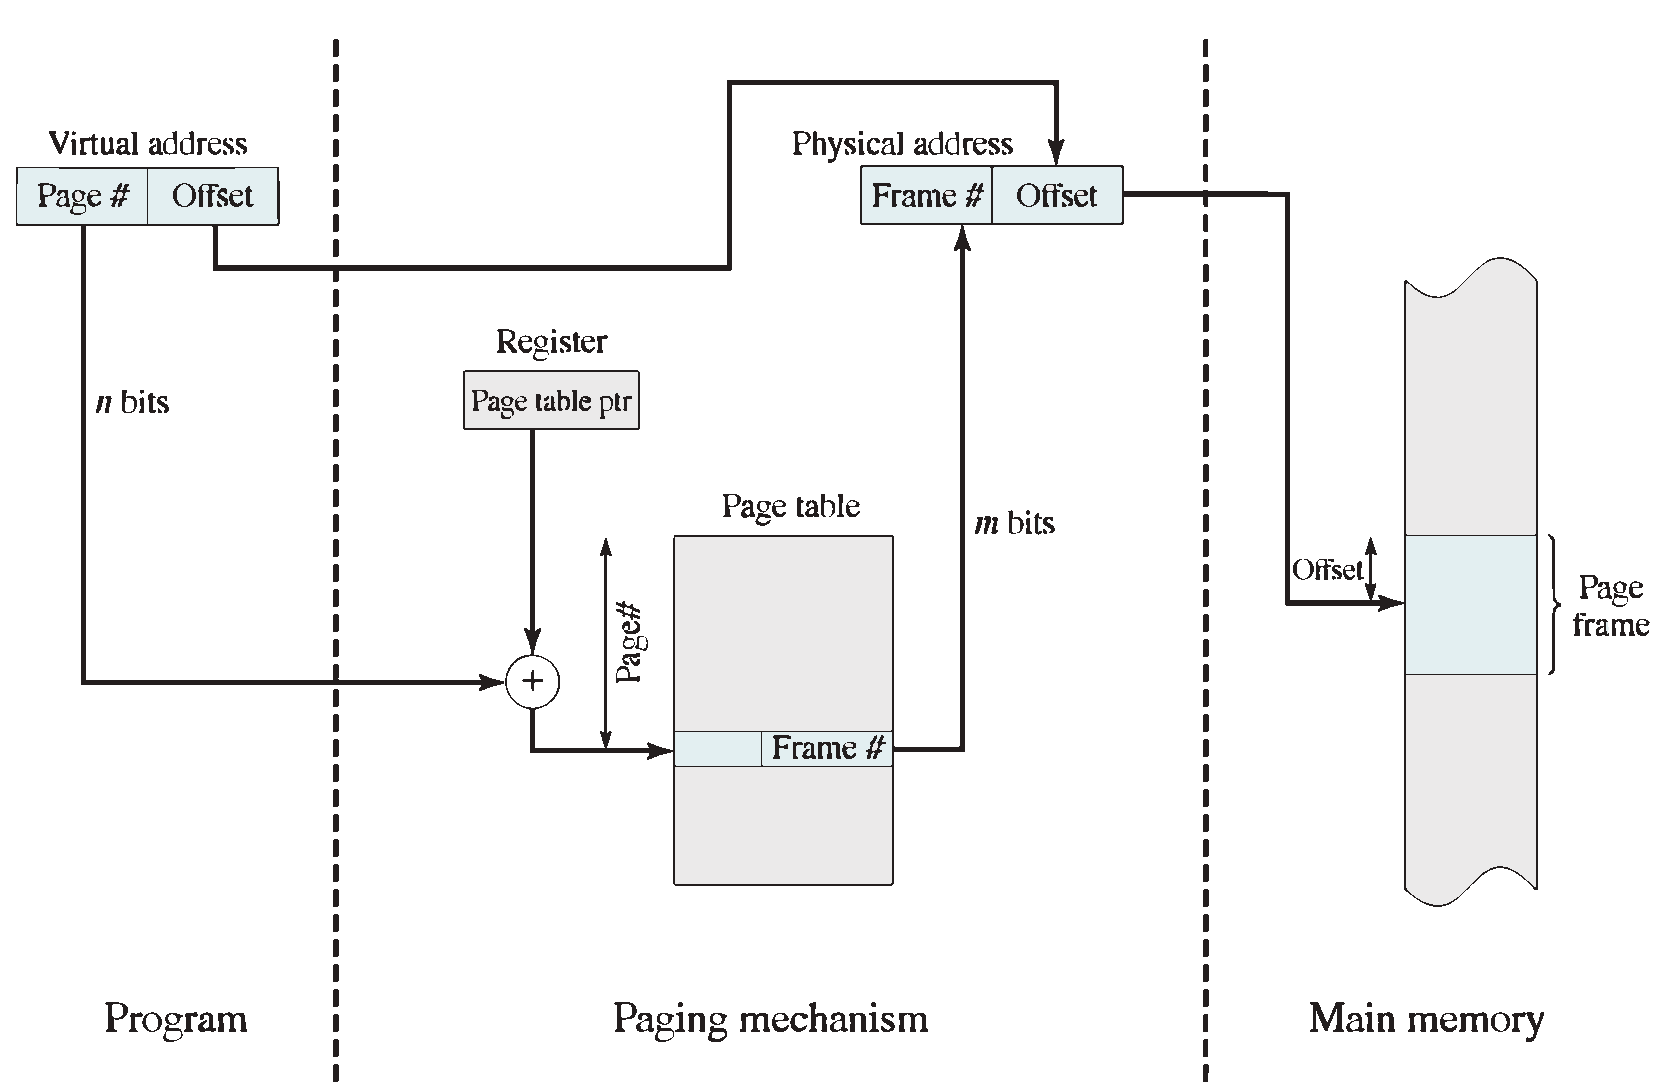
\includegraphics[width=0.80\textwidth]{assets/PagingTraslation.pdf}
    \end{center}
    \caption{Ejemplo de Paginacion}\label{fig:}
\end{figure}

\pagebreak
\subsection{Segmentacion}
\begin{itemize}
    \item Esquema que se asemeja a la "vision del usuario". El programa se divide en partes/secciones.
    \item Un programa es una colecicon de segmentos. Un segmento es una unidad logica, como Programa Ppal, Procedimientos y Funciones, variables locales/globales,etc.
    \item Puede causar fragmentacion.
    \item Todos los segmentos de un programa pueden no tener el mismo tamaño.
    \item Las direcciones logicas consisten en 2 partes:
    \begin{itemize}
        \item Selector de Segmento.
        \item Desplazamiento dentro del segmento. 
    \end{itemize}
    \item \textbf{Tabla de Segmentos:} permite mapear la direccion logica a fisica. Cada entrada contiene:
    \begin{itemize}
        \item Base: Direccion fisica del comienzo del segmento.
        \item Limit: Tamaño del segmento.
    \end{itemize}
    \item Segment-Table base resister (STBR): contiene la direccion de la tabla de segmentos.
    \item Segment-Table length register (STLR): contiene la cantidad de segmentos de un programa.
\end{itemize}
%it just works
\vspace{-0.5cm}
\begin{figure}[h]
    \begin{center}
        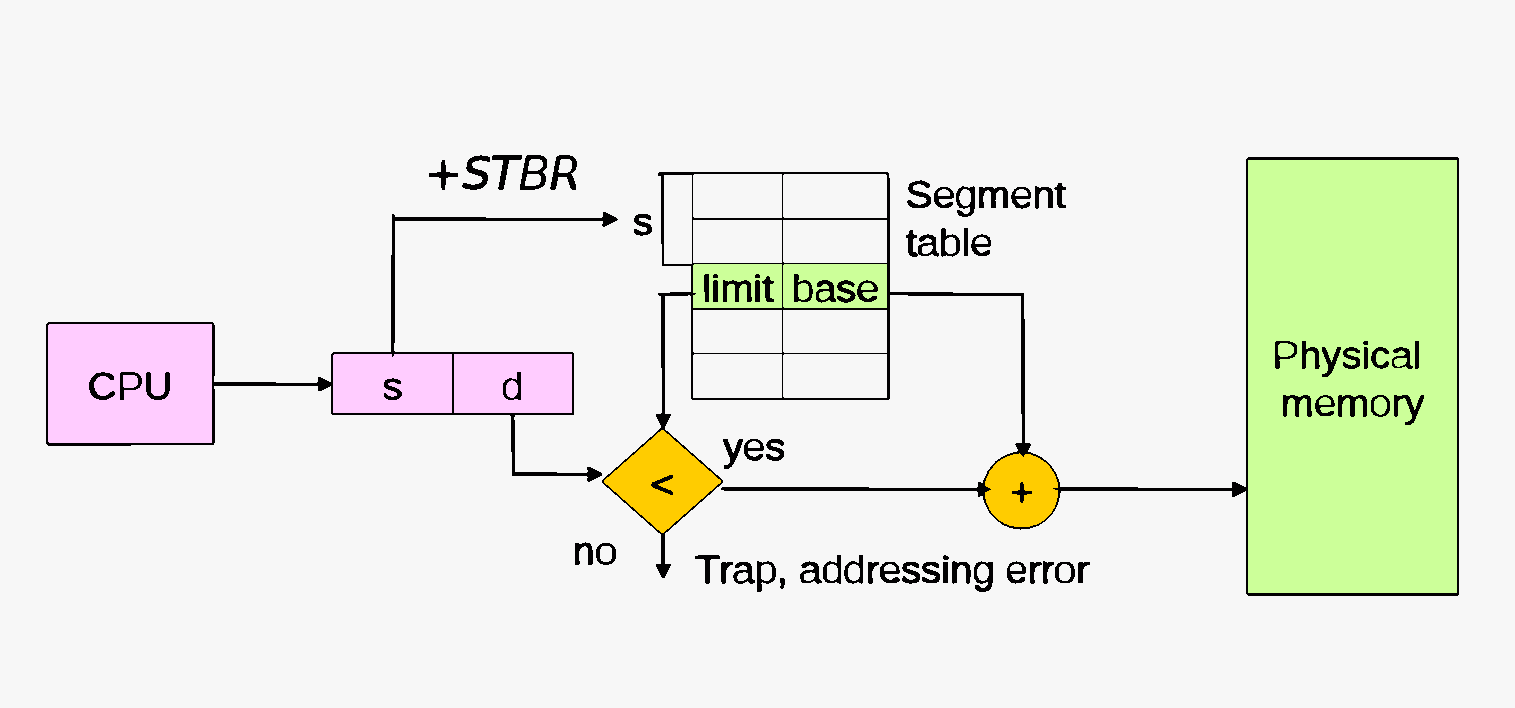
\includegraphics[width=0.90\textwidth]{assets/SegmentationTranslation.pdf}
    \end{center}
    \caption{Traduccion de direcciones en un sistema con Segmentacion}\label{fig:}
\end{figure}
\pagebreak
\subsubsection{Segmentacion Paginada}
\begin{itemize}
    \item La paginacion:
    \begin{itemize}
        \item Transparente al programador.
        \item Elimina Fragmentacion Externa.
    \end{itemize}
    \item La segmentacion:
    \begin{itemize}
        \item Es visible al programador.
        \item Facilita modularidad, estructuras de datos grandes y da mejor soporte a la compraticion y proteccion.
    \end{itemize}
    \item \textbf{Segmentacion Paginada:} cada segmento es dividido en paginas de tamaño fijo.
\end{itemize}
\begin{figure}[h]
    \begin{center}
        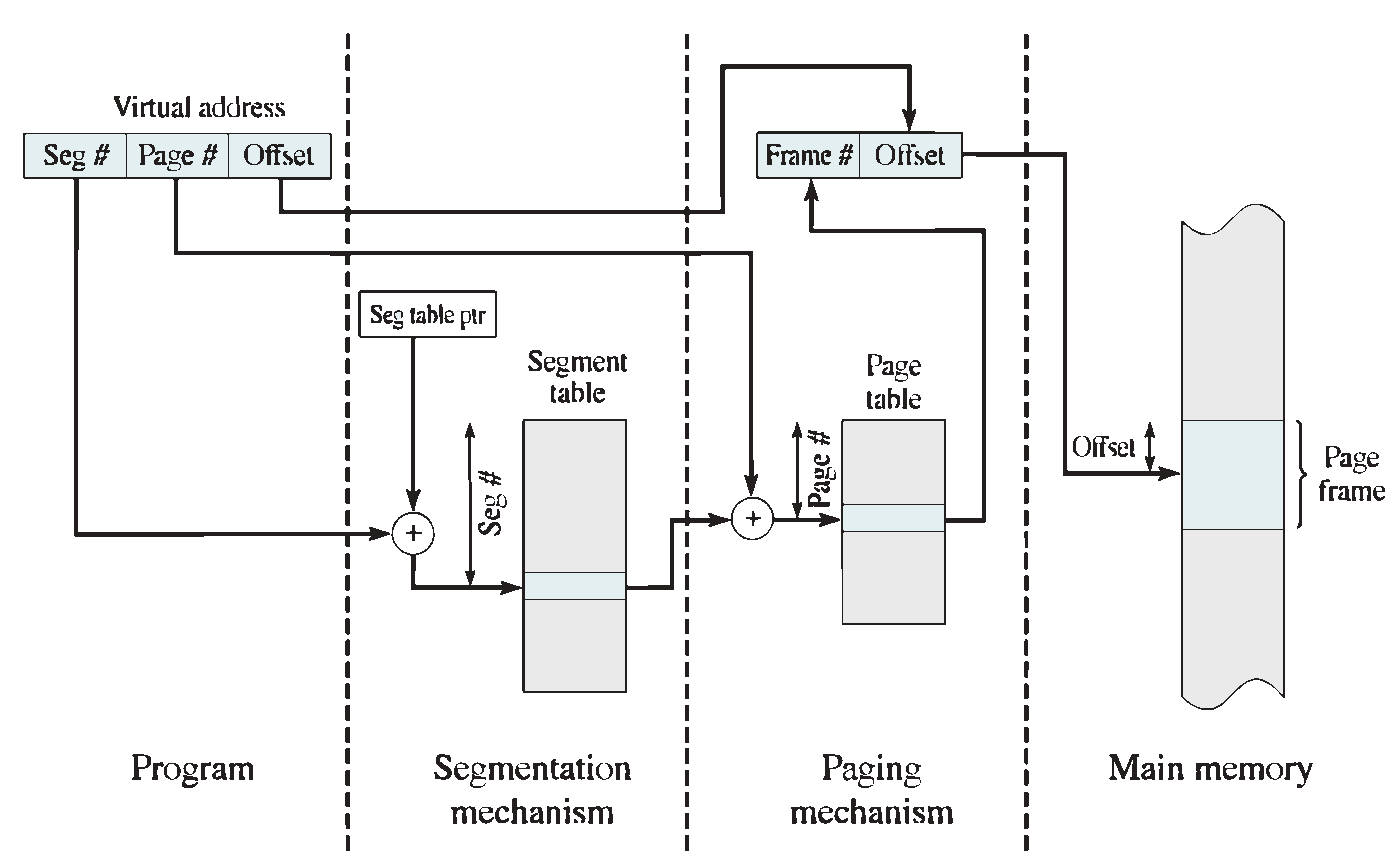
\includegraphics[width=0.95\textwidth]{assets/SegmentacionPaginada.pdf}
    \end{center}
    \caption{Traduccion de direcciones en un sistema con Paginacion Segmentada}\label{fig:}
\end{figure}

